\begin{figure}[t]
      \centering 
      {%\input{example_hole} 
      \scalebox{0.8}{
        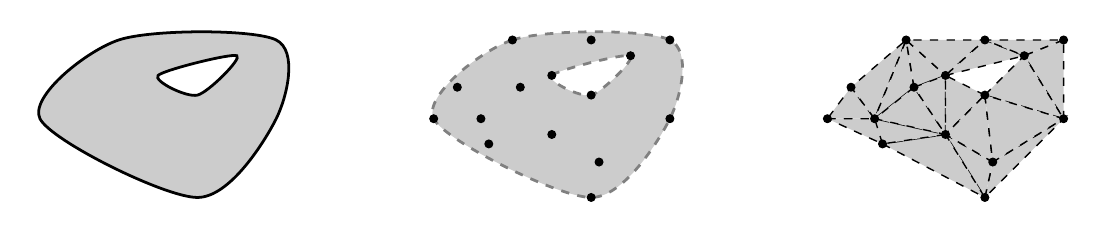
\begin{tikzpicture}
          \draw [black, line width=1, fill=black!20!white] plot [smooth cycle] coordinates {(0,0) (1,1) (3,1) (3,0) (2,-1)};
          \draw [black, line width=1, fill=white] plot [smooth cycle] coordinates {(2.5, 0.8)  (1.5, 0.55) (2, 0.3)     };
      %
      \draw [black!50!white, dashed, line width=1, fill=black!20!white] plot [smooth cycle] coordinates {(5,0) (6,1) (8,1) (8,0) (7,-1)};
          \draw [black!50!white, dashed, line width=1, fill=white] plot [smooth cycle] coordinates {(7, 0.3) (6.5, 0.55) (7.5, 0.8)};
      %
      \draw [black, line width=0.5, fill=black!20!white, circle, dashed  ] (10,0) -- (10.6, 0) -- (10.3, 0.4) -- cycle;
      \draw [black, line width=0.5, fill=black!20!white, circle, dashed  ] (10,0) -- (10.65, 0) -- (10.7, -0.32) -- cycle;
      \draw [black, line width=0.5, fill=black!20!white, circle, dashed  ] (10.6,0) -- (10.3, 0.4) -- (11, 1) -- cycle;
      \draw [black, line width=0.5, fill=black!20!white, circle, dashed  ] (10.6,0) -- (11.1, 0.4) -- (11, 1) -- cycle;
      \draw [black, line width=0.5, fill=black!20!white, circle, dashed  ] (11.5,0.55) -- (11.1, 0.4) -- (11, 1) -- cycle;
      \draw [black, line width=0.5, fill=black!20!white, circle, dashed  ] (11.5,0.55) -- (12, 1) -- (11, 1) -- cycle;
      \draw [black, line width=0.5, fill=black!20!white, circle, dashed  ] (11.5,0.55) -- (12.5, 0.8) -- (12, 1) -- cycle;
      \draw [black, line width=0.5, fill=black!20!white, circle, dashed  ] (13,1) -- (12.5, 0.8) -- (12, 1) -- cycle;
      \draw [black, line width=0.5, fill=black!20!white, circle, dashed  ] (13,1) -- (12.5, 0.8) -- (13, 0) -- cycle;
      \draw [black, line width=0.5, fill=black!20!white, circle, dashed  ] (12,0.3) -- (12.5, 0.8) -- (13, 0) -- cycle;
      \draw [black, line width=0.5, fill=black!20!white, circle, dashed  ] (12,-1) -- (12.1, -0.55) -- (13, 0) -- cycle;
      \draw [black, line width=0.5, fill=black!20!white, circle, dashed  ] (12,-1) -- (12.1, -0.55) -- (11.5, -0.2) -- cycle;
      \draw [black, line width=0.5, fill=black!20!white, circle, dashed  ] (10.7,-0.32) -- (12, -1) -- (11.5, -0.2) -- cycle;
      \draw [black, line width=0.5, fill=black!20!white, circle, dashed  ] (10.7,-0.32) -- (10.6, 0) -- (11.5, -0.2) -- cycle;
      \draw [black, line width=0.5, fill=black!20!white, circle, dashed  ] (11.1, 0.4) -- (10.6, 0) -- (11.5, -0.2) -- cycle;
      \draw [black, line width=0.5, fill=black!20!white, circle, dashed  ] (11.1, 0.4) -- (11.5, 0.55) -- (11.5, -0.2) -- cycle;
      \draw [black, line width=0.5, fill=black!20!white, circle, dashed  ] (12, 0.3) -- (11.5, 0.55) -- (11.5, -0.2) -- cycle;
      \draw [black, line width=0.5, fill=black!20!white, circle, dashed  ] (12, 0.3) -- (12.1, -0.55) -- (11.5, -0.2) -- cycle;
      \draw [black, line width=0.5, fill=black!20!white, circle, dashed  ] (12, 0.3) -- (12.1, -0.55) -- (13, 0) -- cycle;
      %   
      \node [draw=black,fill=black, shape=circle, scale=0.3] at (10, 0) {};
      \node [draw=black,fill=black, shape=circle, scale=0.3] at (11.1, 0.4) {};
      \node [draw=black,fill=black, shape=circle, scale=0.3] at (11.5, 0.55) {};
      \node [draw=black,fill=black, shape=circle, scale=0.3] at (11.5, -0.2) {};
      \node [draw=black,fill=black, shape=circle, scale=0.3] at (12, 0.3) {};
      \node [draw=black,fill=black, shape=circle, scale=0.3] at (12.1, -0.55) {};
      \node [draw=black,fill=black, shape=circle, scale=0.3] at (13, 0) {};
      \node [draw=black,fill=black, shape=circle, scale=0.3] at (10.7, -0.32) {};
      \node [draw=black,fill=black, shape=circle, scale=0.3] at (10.6, 0) {};
      \node [draw=black,fill=black, shape=circle, scale=0.3] at (12, -1) {};
      \node [draw=black,fill=black, shape=circle, scale=0.3] at (12.5, 0.8) {};
      \node [draw=black,fill=black, shape=circle, scale=0.3] at (10.3, 0.4) {};
      \node [draw=black,fill=black, shape=circle, scale=0.3] at (11, 1) {};
      \node [draw=black,fill=black, shape=circle, scale=0.3] at (12, 1) {};
      \node [draw=black,fill=black, shape=circle, scale=0.3] at (13, 1) {};
      %  
      \node [draw=black,fill=black, shape=circle, scale=0.3] at (5, 0) {};
      \node [draw=black,fill=black, shape=circle, scale=0.3] at (6.1, 0.4) {};
      \node [draw=black,fill=black, shape=circle, scale=0.3] at (6.5, 0.55) {};
      \node [draw=black,fill=black, shape=circle, scale=0.3] at (6.5, -0.2) {};
      \node [draw=black,fill=black, shape=circle, scale=0.3] at (7, 0.3) {};
      \node [draw=black,fill=black, shape=circle, scale=0.3] at (7.1, -0.55) {};
      \node [draw=black,fill=black, shape=circle, scale=0.3] at (8, 0) {};
      \node [draw=black,fill=black, shape=circle, scale=0.3] at (5.7, -0.32) {};
      \node [draw=black,fill=black, shape=circle, scale=0.3] at (5.6, 0) {};
      \node [draw=black,fill=black, shape=circle, scale=0.3] at (7, -1) {};
      \node [draw=black,fill=black, shape=circle, scale=0.3] at (7.5, 0.8) {};
      \node [draw=black,fill=black, shape=circle, scale=0.3] at (5.3, 0.4) {};
      \node [draw=black,fill=black, shape=circle, scale=0.3] at (6, 1) {};
      \node [draw=black,fill=black, shape=circle, scale=0.3] at (7, 1) {};
      \node [draw=black,fill=black, shape=circle, scale=0.3] at (8, 1) {};
      %
      
        \end{tikzpicture}
        }
      }
      \caption{Continuous and analogous discrete manifolds with one $1$-dimensional hole ($\dim \bar{\mc H}_1=1$). Left pane: the continuous manifold; center pane: the discretization with mesh vertices; right pane: a simplicial complex built upon the mesh. Triangles in the simplicial complex $\mc K$ are colored gray (right). 
      \label{fig:example_holes}
      }
    \end{figure}
    